\documentclass[../main.tex]{subfiles}

\begin{document}

\chapter{Об’єктно-орієнтоване проектування ІС}

Якщо аналіз об’єкта проектування – це розробка відповідної логічної моделі, яка описує усі можливі та прийнятні варіанти розв’язання задач, які вказують, що повинна робити система, то проектування – це вироблення рішення відповідно до моделі аналізу, яке оптимізує набір критеріїв проектування, які  показують, як ця поведінка (робота) системи може бути реалізована \cite{diploma_guidelines}.
Оскільки, у даній роботі застосовується об’єктно-орієнтована технологія проектування, то проектна частина повинна складатися із таких етапів:

\begin{enumerate}
	\item Архітектурне проектування – описує логічну структуру інформаційної системи (програмні класи, підсистеми,  пакети) та їх зв’язки.
	\item Детальне проектування – описує структури даних та алгоритми всередині окремих класів. 
\end{enumerate}

\section{Архітектурне проектування}
Формування архітектури – перший і основний крок у розв’язанні завдання проектування, що закладає фундамент уявлення програмної системи, здатної виконувати весь спектр детальних вимог. \cite{diploma_guidelines2}

Створення архітектури – це проектування на найвищому рівні (логічна архітектура). Логічна архітектура описує систему в термінах її принципової організації у вигляді пакетів, програмних класів і підсистем. Вона називається логічною, оскільки не визначає способи розгортання цих елементів у різних операційних системах або на фізичних комп’ютерах в мережі (це відноситься до архітектури розгортання) \cite{diploma_guidelines}.

Система Android надає різнобічну платформу додатків, на основі якої можна створювати інноваційні програми та ігри для мобільних пристроїв в середовищі мови Java. Важливо знати наступні основні концепції, що стосуються платформи додатків Android.

\textbf{Додатки мають кілька точок входу.} 
Додатки для Android будуються з окремих компонентів, які можна викликати незалежно один від одного. Наприклад, окрема операція надає один екран для користувацького інтерфейсу, а служба незалежно виконує роботу у фоновому режимі.
	
За допомогою об'єкта Intent з одного компонента можна запустити інший. Також можна запустити компонент з іншої програми, наприклад, операцію з картографічного додатка, щоб показати адресу. Ця модель формує кілька точок входу для однієї програми, і при цьому користувач може вибрати будь-який додаток за замовчуванням для виконання тієї чи іншої дії, яка може викликати інші додатки.
	
\textbf{Додатки адаптуються до різних пристроїв.} 
Android надає адаптивну платформу додатків, яка дозволяє забезпечувати унікальні ресурси для різних конфігурацій пристроїв. Наприклад, можна створити різні файли XML макета для екранів різних розмірів, а система буде визначати, який макет використовувати, з урахуванням розміру екрану даного пристрою.

Якщо якимось функціям програми потрібне певне обладнання, наприклад камера, можна запитувати його наявність в пристрої під час виконання. При необхідності також можна оголошувати функції, які потрібні додатку, для того, щоб такі магазини додатків, як Google Play, не дозволяли встановлювати додатки на пристроях, в яких цих функцій немає.

\subsection{Компоненти Android-додатку}

Компоненти програми є частинками, з яких складається додаток для Android. Кожен компонент являє собою окрему точку, через яку система може увійти в додаток. Не всі компоненти є точками входу для користувача, а деякі з них залежать один від одного. При цьому кожен компонент є самостійною структурною одиницею і відіграє певну роль -- кожен з них являє собою унікальний елемент структури, який визначає роботу програми в цілому.

Компоненти програми можна віднести до одного з чотирьох типів. Компоненти кожного типу призначені для певної мети, вони мають власний життєвий цикл, який визначає спосіб створення і припинення існування компонента.

\textbf{Операції.} Операція (Activity) являє собою один екран з користувацьким інтерфейсом. Наприклад, в додатку для роботи з електронною поштою одна операція може служити для відображення списку нових повідомлень, інша -- для створення повідомлення і третя операція -- для читання повідомлень. Незважаючи на те, що операції спільно формують чітку взаємодію користувача з додатком по роботі з електронною поштою, кожна з них не залежить від інших операцій. Будь-які з цих операцій можуть бути запущені іншим додатком (якщо додаток дозволяє це). Наприклад, додаток для камери може запустити операцію в додатку по роботі з електронною поштою, яка створює нове повідомлення, щоб користувач міг відіслати фотографію.

\textbf{Служби.} Служба (Service) являє собою компонент, який працює у фоновому режимі і виконує тривалі операції, пов'язані з роботою віддалених процесів. Служба не має користувацього інтерфейсу. Наприклад, вона може відтворювати музику у фоновому режимі, поки користувач працює в іншому додатку, або може отримувати дані по мережі, не блокуючи взаємодію користувача з операцією. Служба може бути запущена іншим компонентом, який потім буде взаємодіяти з нею.

\textbf{Постачальники контенту.} Постачальник контенту (Content provider) управляє загальним набором даних програми. Дані можна зберігати в файловій системі, базі даних, інтернеті або будь-якому іншому постійному місці зберігання, до якого у додатка є доступ. За допомогою постачальника контенту інші додатки можуть запитувати або навіть змінювати дані (якщо постачальник контенту дозволяє робити це). Наприклад, в системі Android є постачальник контенту, який управляє інформацією контактів користувача. Будь-який додаток, що отримав відповідні дозволи, може запитати частину цього постачальника контенту, для читання і запису відомостей про певну людину.

\textbf{Приймачі широкомовних повідомлень.} Приймач широкомовних повідомлень (Broadcast receiver) являє собою компонент, який реагує на оголошення поширювані по всій системі. Багато з цих оголошень розсилає система -- наприклад, оголошення про те, що екран вимкнувся, акумулятор розряджений або був зроблений фотознімок. Оголошення також можуть розсилатися додатками, наприклад, щоб повідомити іншу програму про те, що якісь дані були завантажені на пристрій і тепер готові для використання. Незважаючи на те, що приймачі широкомовних повідомлень не мають інтерфейсу користувача, вони можуть створювати повідомлення в рядку стану, щоб попередити користувача про подію. Однак, найчастіше вони є просто шлюзом для інших компонентів і призначені для виконання мінімального обсягу роботи. Наприклад, вони можуть ініціювати виконання службою певних дій при виникненні події.

Унікальною особливістю системи Android є те, що будь-який додаток може запустити компонент іншого додатку. Наприклад, якщо розробник хоче дати користувачеві можливість фотографувати, використовуючи камеру пристрою, то, якщо є інший додаток, який може виконати цю дію, замість того щоб розробити операцію фотографування в своєму додатку, він може викликати такий додаток. Не потрібно впроваджувати код з програми для камери або навіть встановлювати на нього посилання. Замість цього можна просто запустити операцію фотографування з програми для камери. По завершенні цієї операції фотографія буде повернута в додаток, і її можна буде використовувати. Для користувача це буде виглядати як один додаток.

Коли система запускає компонент, вона запускає процес для цього додатка (якщо він ще не був запущений) і створює екземпляри класів, які потрібні цьому компоненту. Наприклад, якщо додаток запустить операцію фотографування в додатку для камери, ця операція буде виконуватися в процесі, який відноситься до цього стороннього додатку. Тому, на відміну від додатків для більшості інших систем, в додатках для Android відсутня єдина точка входу.

Оскільки система виконує кожен додаток в окремому процесі з правами доступу до файлів, які обмежують доступ до інших додатків, він не може безпосередньо викликати компонент з іншого додатку. Це може зробити сама система Android. Тому, щоб викликати компонент в іншому додатку, необхідно повідомити системі про свій намір (Intent) запустити певний компонент. Після цього система активує для цей компонент.

Для запуску компонента додатку системі Android необхідно знати, що компонент існує. Для цього вона читає файл маніфесту додатка (AndroidManifest.xml). У цьому файлі, який повинен знаходитися в кореневій теці програми, повинні бути оголошені всі компоненти програми.

\subsection{Подубова діаграми пакетів}
Одним з важливих етапів архітектурного проектування є побудова діаграми пакетів. Діаграма пакетів є діаграмою, яка містить пакети класів і залежності між ними. Вона описує архітектурну основу системи і допомагає в управлінні масштабами і складністю системи. 

Діаграма пакетів для додатку зображена на рис. \ref{diagram:packages}.
\vspace{\baselineskip}

\begin{figure}[H]
	\centering
	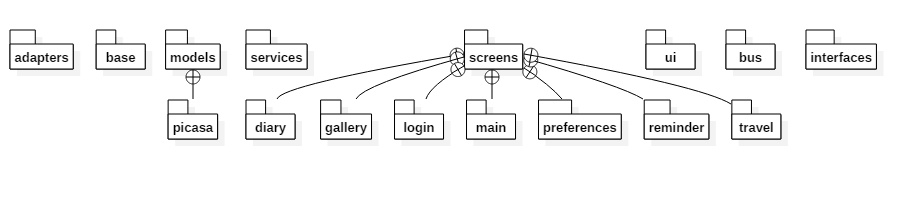
\includegraphics[width=1\textwidth]{diagram_packages}
	\caption{Діаграма пакетів для Android-щоденника}
	\label{diagram:packages}
\end{figure}

Пакет \textit{\textbf{adapters}} призначений для адаптерів. Адаптер -- це об'єкт, що діє як міст між предсталенням (view) і даними для цього представлення. Він забезпечує доступ до елементів даних. Також, адаптер відповідальний за подання представлення для кожного елемента в наборі даних \cite{adapter}. 

В пакеті \textit{\textbf{models}} будуть знаходитися класи моделей, що необхідні для взаємодії з базою даних чи іншими сервісами. Пакет \textit{\textbf{screens}} призначений для класів операцій, що являють собою окремі екрани додатку, тому в нього були додані додаткові пакети, щоб розділити екрани по областях, за які вони відповідають. Пакет \textit{\textbf{services}} буде містити служби, а пакети \textit{\textbf{ui}}, \textit{\textbf{bus}} та \textit{\textbf{interfaces}} -- компоненти, що відповідають за інтерфейс користувача, шину подій та Java інтерфейси відповідно. 

\subsection{Побудова діаграми компонентів}

Ще одним будівельним блоком для створення архітектури об'єктно-орієнтованої системи вважається компонент. Діаграма компонентів показує розбиття програмної системи на структурні компоненти та залежності між компонентами. В якості фізичних компонентів можуть бути файли, бібліотеки, модулі, виконувані файли, пакети і т.п. У багатьох середовищах розробки модуль або компонент відповідає файлу. Стрілки, що з'єднують модулі, показують відносини взаємозалежності аналогічні тим, які мають місце при компіляції вихідних текстів програм. Основними графічними елементами діаграми компонентів є компоненти, інтерфейси і залежності між ними. 

Діаграму компонентів для Android-щоденника зображено на рис. \ref{diagram:hierarchy}.

%TODO: describe this

\begin{figure}[H]
	\centering
	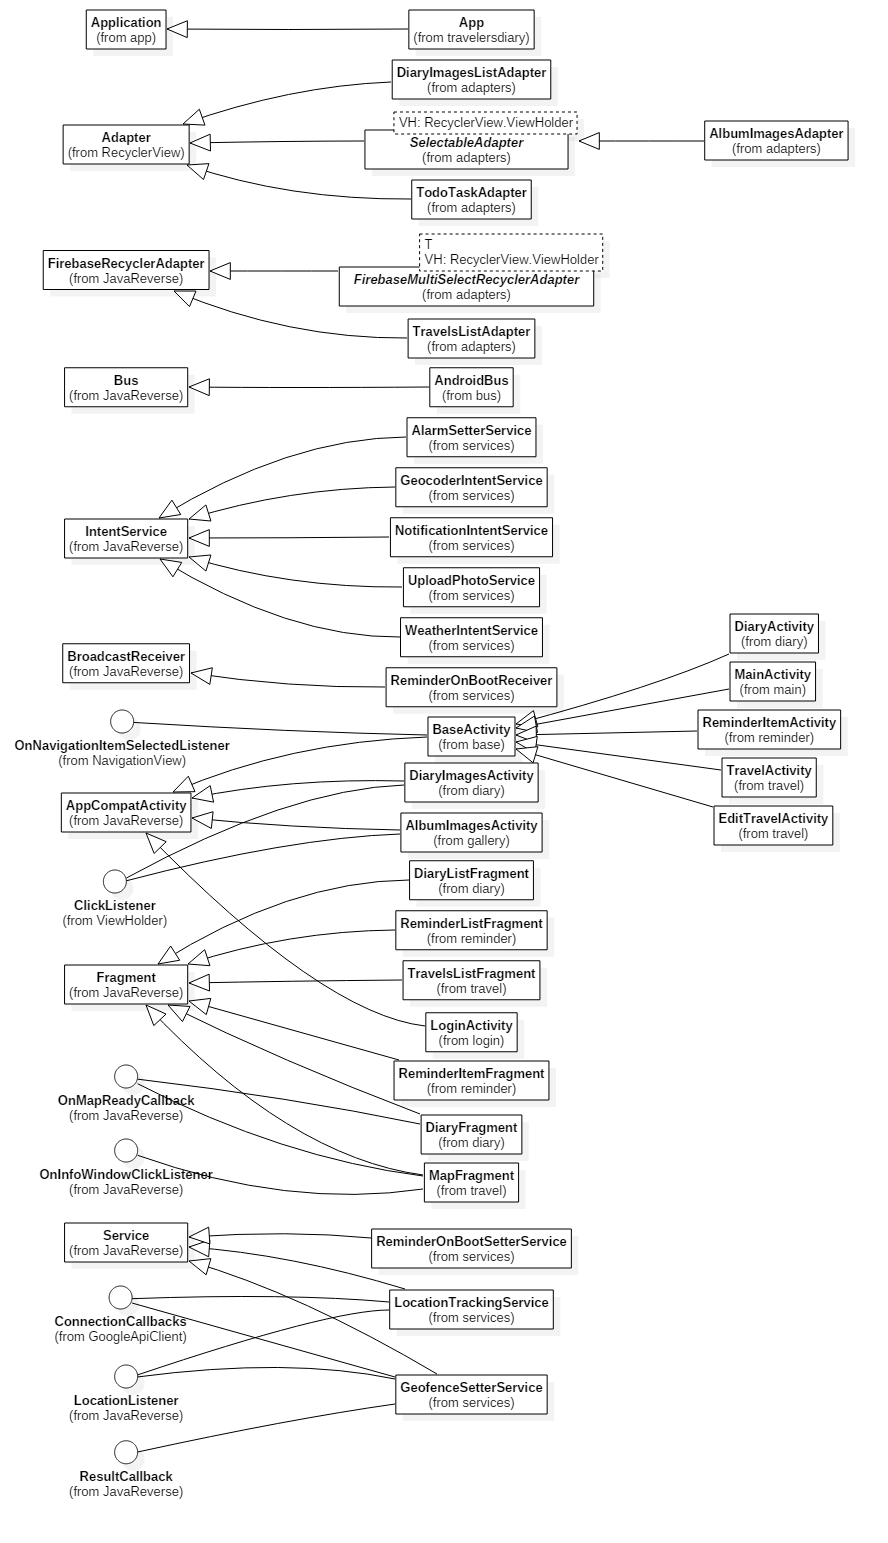
\includegraphics[height=0.8\textheight]{diagram_hierarchy}
	\caption{Діаграма компонентів Android-щоденника}
	\label{diagram:hierarchy}
\end{figure}

\section{Детальне проектування}

Детальне проектування – описує структури даних та алгоритми всередині окремих класів [10]. 

У програмуванні структури даних ‒ це способи організації даних в комп’ютерах. Часто разом зі структурою даних пов’язується і специфічний перелік операцій, які можуть бути виконаними над даними.
Правильний підбір структур даних є надзвичайно важливим для ефективного функціонування відповідних алгоритмів їх обробки. Добре побудовані структури даних дозволяють оптимізувати використання машинного часу та пам’ятті комп’ютера для виконання найбільш критичних операцій.

Логічна будова інформаційної системи (див. рис. \ref{diagram:models}) побудована  за допомогою UML-діаграми класів, яка служить для представлення статичної структури моделі системи в термінології класів об’єктно-орієнтованого програмування.

\begin{figure}[H]
	\centering
	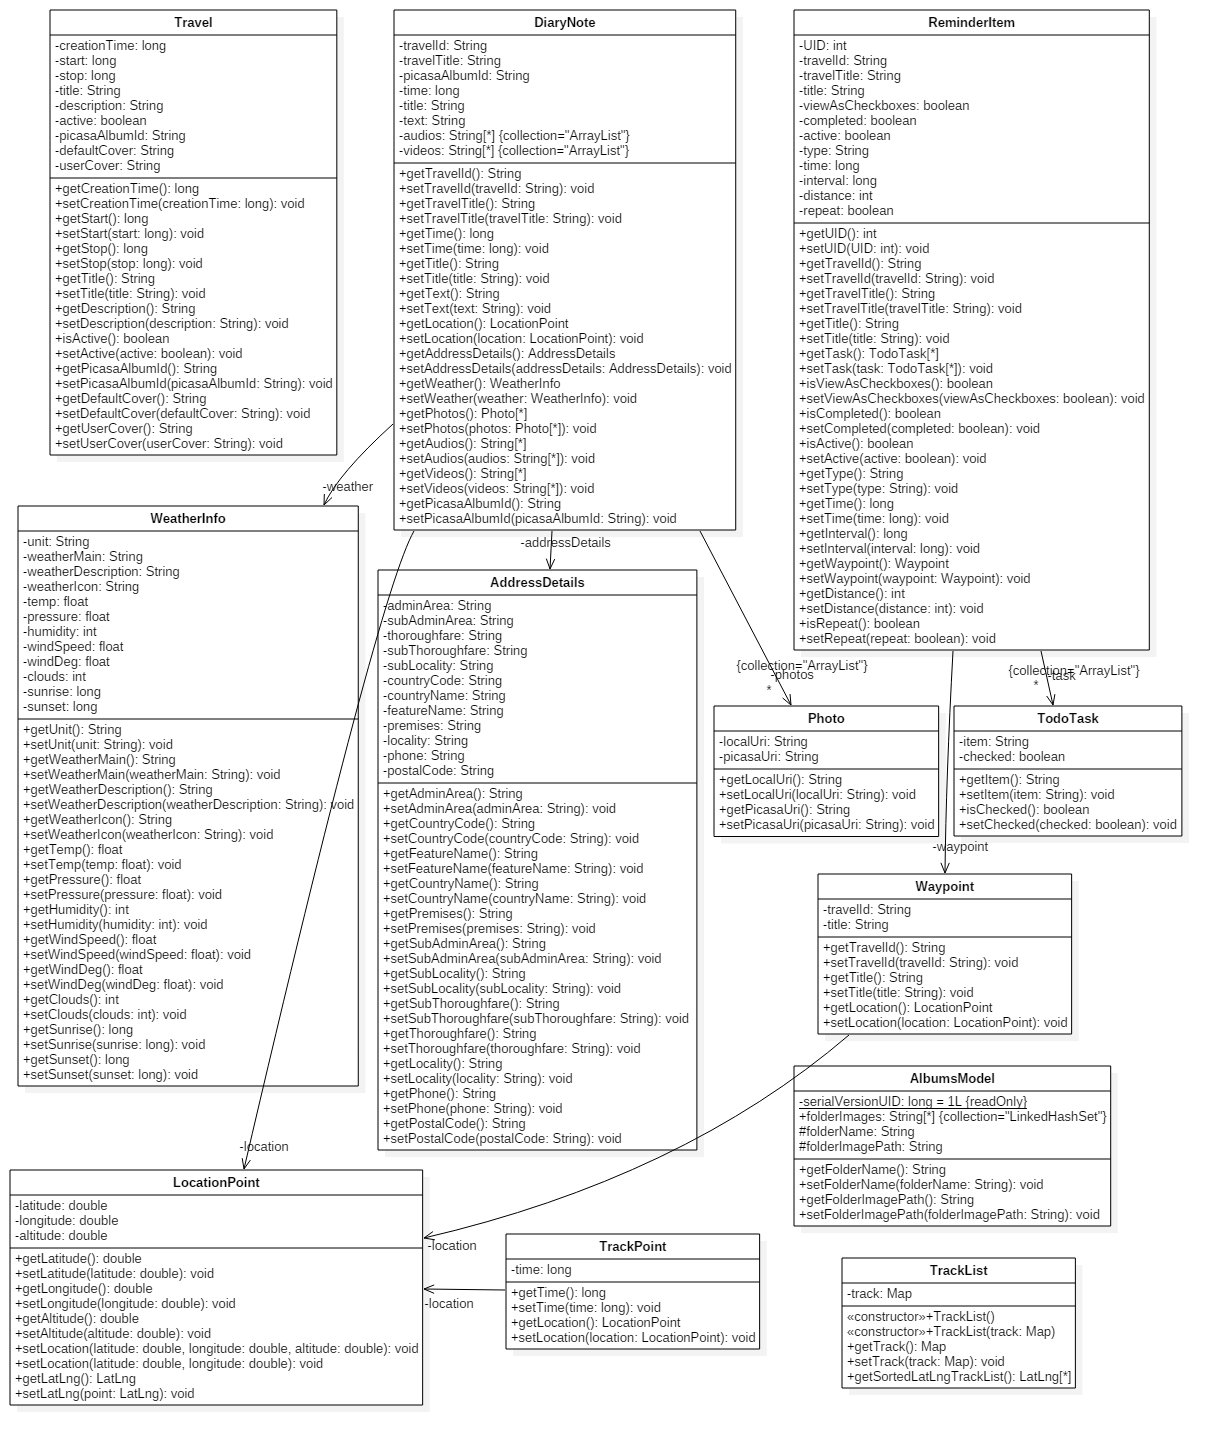
\includegraphics[height=0.8\textheight]{diagram_models}
	\caption{Діаграма моделей Android-щоденника}
	\label{diagram:models}
\end{figure}

Дані моделі використовуються для збереження об'єктів до бази даних та їх отримання.

%TODO: add models description

\section{Розгортання програмної системи на апаратних засобах}

Для функціонування додатку необхідна операційна система Android версії 4.2 (API 16) і вище.

%TODO: add something here

\section{Висновки}

%TODO: Висновки до розділу (не більш 1-2 сторінки). Розмір одного висновку приблизно – один абзац (5-7 рядків). Висновки цього розділу є важливою і значущою частиною роботи.

\end{document}